\documentclass[12pt, twoside, exarticle]{article}
\usepackage[left=28mm, top=24mm, right=28mm, bottom=24mm, asymmetric, reversemarginpar]{geometry}
\usepackage{titlesec}
\usepackage{marginnote}
\usepackage{listings}
\usepackage{color}
\usepackage{xkeyval}
\usepackage{varwidth}
\usepackage{microtype}
\usepackage{hyperref}
\usepackage{enumerate}
\usepackage{graphicx}
\title{\textbf{CS240 Review Notes}}
% Code box.
\lstnewenvironment{code}[1][]
	{\begingroup
		%\vfil\penalty-9999\vfilneg\lstset{language=#1}
		\lstset{language=#1}
	}
	{\endgroup}

% Definition box.
\newcommand{\defnbox}[2] {
	\setlength{\fboxsep}{8pt}
	\marginpar {
		\vspace{0.9em}
		\begin{center}
		\footnotesize{\textbf{\color{brown}DEFINITION}}
		\footnotesize{\textbf{#1}}
		\end{center}
	}
	\colorbox{lightyellow}{
		\begin{minipage}{\dimexpr\linewidth-2\fboxsep}
		#2
		\end{minipage}
	}
	~\\
}

% Example box.
\newcommand{\exbox}[2] {
	\setlength{\fboxsep}{8pt}
	\marginpar {
		\vspace{0.9em}
		\footnotesize{\textbf{\color{darkpurple}EXAMPLE #1}}
	}
	\colorbox{lightpurple}{
		\begin{minipage}{\dimexpr\linewidth-2\fboxsep}
		#2
		\end{minipage}
	}
	~\\
}

% Exercise box.
\newcommand{\exerbox}[1] {
	\setlength{\fboxsep}{8pt}
	\marginpar {
		\vspace{0.9em}
		\footnotesize{\textbf{\color{darkred}EXERCISE}}
	}
	\colorbox{lightred}{
		\begin{minipage}{\dimexpr\linewidth-2\fboxsep}
		#1
		\end{minipage}
	}
	~\\
}

% Used on the side for definitions.
\definecolor{brown}{RGB}{101, 91, 71}
\definecolor{lightyellow}{RGB}{228, 224, 128}

% Used for the code block itself.
\definecolor{codebg}{RGB}{255, 255, 238}
\definecolor{codeborder}{RGB}{243, 242, 222}

% Used for exercises.
\definecolor{darkred}{RGB}{203, 20, 20}
\definecolor{lightred}{RGB}{229, 130, 130}

% Used for examples.
\definecolor{darkpurple}{RGB}{76, 60, 189}
\definecolor{lightpurple}{RGB}{184, 183, 255}

% Used for C and Lisp Syntax.
\definecolor{purple}{RGB}{174, 19, 198}
\definecolor{darkblue}{RGB}{0, 0, 102}
\definecolor{lightblue}{RGB}{50, 155, 171}
\definecolor{lightgreen}{RGB}{29, 131, 43}

% Document formatting for headings.
\pagestyle{myheadings}
\setcounter{secnumdepth}{4} % 4 being sub sections.

% Removes indentation of paragraphs.
\setlength{\parindent}{0cm}

% Sets page numbering to roman.
\pagenumbering{roman}

% Declaring the default listing style.
\lstdefinestyle{default_style} {
	backgroundcolor=\color{codebg},
	rulecolor=\color{codeborder},
	stringstyle=\color{purple},
	keywordstyle=\color{darkblue},
	identifierstyle=\color{lightblue},
	commentstyle=\color{lightgreen},
	basicstyle=\footnotesize\sffamily,
	xleftmargin=10pt,
	xrightmargin=10pt,
	belowcaptionskip=10pt,
	belowskip=20pt,
	framesep=10pt,
	frame=single,
	%numbers=left,
	%numbersep=8pt,
	showspaces=false,
	showstringspaces=false,
	tabsize=2
}

% Sets the default style for all code blocks.
\lstset {
	style=default_style
}

% Module section shortcut commands.
\newcommand{\newpagesection}[1] {
	\clearpage
	\section{#1}
}

\newcommand{\newpagesubsection}[1] {
	\clearpage
	\subsection{#1}
}
\begin{document}
\makeatletter
\hfil\parbox[t]{0.7\textwidth}{\centering\LARGE\bfseries\@title}\par
\kern0.5cm \hrule\kern0.5cm
\makeatother

% Table of contents
\renewcommand{\contentsname}{Table of Contents}
\tableofcontents
\clearpage

% Content
\pagenumbering{arabic}
\setlength{\oddsidemargin}{1.6cm}
\setlength{\evensidemargin}{\oddsidemargin}
\setlength{\marginparwidth}{2.6cm}
\setlength{\marginparsep}{0.25cm}

\newpagesection{Computer Abstractions}

Lecture 1 was spend worrying about a bunch of course administration stuff you already know about, so the material started in lecture 2. \\

\subsection{The Computer Revolution}

Technology, as you must know by now, is an ever developing beast.  Moore's law states that computation power doubles every two years and actually, it's been pretty damn accurate.  Today we have computers in everything, and smaller than ever.  As computers have become more pervasive, classes of computers have emerged:
\begin{itemize}
\item Desktop computers (includes desktops)
	\begin{itemize}
	\item General purpose, variety of software.
	\item Subject to cost/performance trade-off.
	\item Thought as the ``first consumer computers''.
	\end{itemize}
\item Server computers
	\begin{itemize}
	\item Network based.
	\item High capacity, performance, reliability.
	\item Range from small servers to building sized.
	\end{itemize}
\item Embedded computers
	\begin{itemize}
	\item Hidden as components of systems.
	\item Stringent power/performance/cost constraints.
	\end{itemize}
\end{itemize}

\subsection{Components of a Computer}

Computers themselves are like an onion.  You write applications that then communicate with the system software (Operating system) which then interacts with the hardware.  If we were to always just write applications that communicate with the hardware, we would need to adapt the code for every different kind of hardware configuration.  This could even mean something as simple as 4GB of RAM or 8.  This intermediary step of communication with an operating system will make you program a little slower, but the benefits greatly outweigh the cost. \\

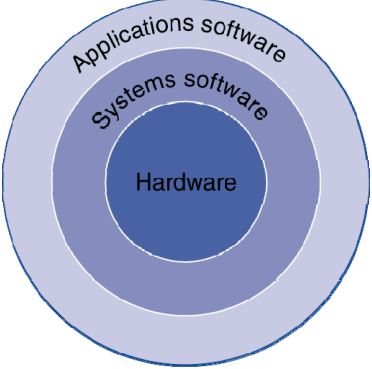
\includegraphics{graphics/onioncomputer.png}

\subsubsection{Memory}

Memory is where the computer stores its information.  Memory could be RAM (random access memory), the processor cache (quickly accessible memory inside the processor) or even hard drive disk. \\

In theory, we can have perfect memory which is:
\begin{itemize}
\item Fast
\item Large
\item Cheap
\end{itemize}

In reality, you can only chose two from the above list.  For instance it would be incredibly to have a large processor cache, but in reality this is extremely cost prohibitive. \\

\subsubsection{CPU}

The CPU (central processing unit) is the brains of the computer.  It consists of three important parts.
\begin{enumerate}
\item Datapath
	\begin{itemize}
	\item The stream of information coming into the CPU.
	\end{itemize}
\item Control Unit
	\begin{itemize}
	\item TIn charge of sequencing the datapath and memory.  It decided which process gets precedence over another.  The actual ``brain'' of the processor.
	\end{itemize}
\item Cache Memory
	\begin{itemize}
	\item Small amount of memory that can be accessed instantly (the same clock cycle as the computation).  These are often layered and names L1, L2 and L3 with L1 being the easiest to access.
	\end{itemize}		
\end{enumerate}

Here's a picture of a typical processor with the first core ``opened up'' to see its internal structure. \\

\scalebox{0.65}{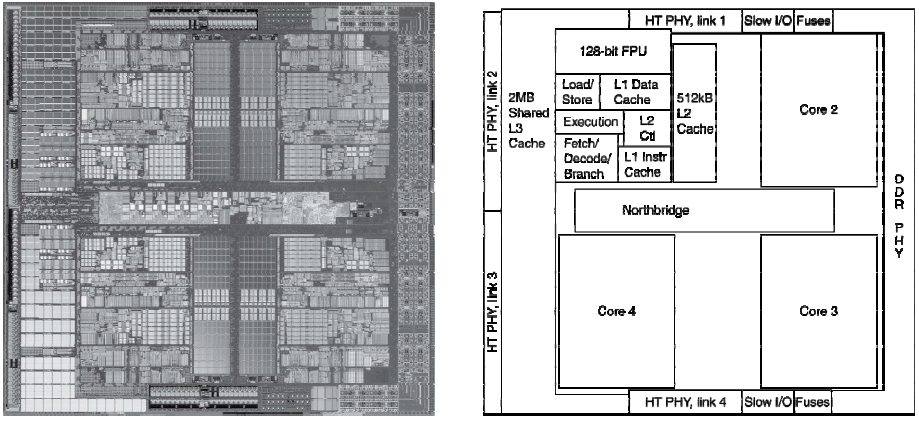
\includegraphics{graphics/processorcore.png}}



\end{document}